\Exercise[number={1}]
A variable \(x\) in \(\mathbf{R}\) (scalar) is emitted by two possible sources,
\(w_1\), \(w_2\) with probability \(Pr(w_1)=Pr(w_2)=0.5\). 
We intend to design a Bayes classifier that assigns the correct class to each
observed \(x\). If the \(p(x|w_i)\) both have a Gaussian distribution, with
mean \(\mu_i\) and different variances \(\sigma_i^2\), determine the
boundaries of the decision regions as \(h=\sigma_2^2 / \sigma_1^2\)
varies.

\Answer[number={1}]
The boundaries of a binary classifier can be studied by computing the
sign of \(z(x)\), with \(z\) being the exponent of the sigmoid function, in
particular the decision boundaries are given by \(z(x)=0\).
\begin{align*}
    z(x)
    &=\log{\frac{p(x|w_1)}{p(x|w_2)}} + \log{\frac{Pr(w_1)}{Pr(w_2)}}
    =\log{p(x|w_1)}-\log{p(x|w_2)}+\cancel{\log{\frac{0.5}{0.5}}}\\
    &=-\frac{1}{2}\log{(2\pi\sigma_1^2)}-\frac{1}{2\sigma_1^2}(x-\mu_1)^2+\frac{1}{2}\log{(2\pi\sigma_2^2)}+\frac{1}{2\sigma_2^2}(x-\mu_2)^2\\
    &=\frac{1}{2}\log{\biggl(\frac{\cancel{2\pi}\sigma_2^2}{\cancel{2\pi}\sigma_1^2}\biggr)}+\frac{1}{2}\biggl(\frac{x^2+\mu_2^2-2\mu_2x}{\sigma_2^2}-\frac{x^2+\mu_1^2-2\mu_1x}{\sigma_1^2}\biggr)
\end{align*}
\begin{align*}
    z(x)=0 \Longleftrightarrow \cancel{\frac{1}{2}}\log{\biggl(\frac{\sigma_2^2}{\sigma_1^2}\biggr)}+\cancel{\frac{1}{2}}\biggl(\frac{x^2+\mu_2^2-2\mu_2x}{\sigma_2^2}-\frac{x^2+\mu_1^2-2\mu_1x}{\sigma_1^2}\biggr)=0
\end{align*}
\begin{align*}
    \Rightarrow
    \biggl(\frac{1}{\sigma_2^2}-\frac{1}{\sigma_1^2}\biggr)x^2+
    2\biggl(\frac{\mu_1}{\sigma_1^2}-\frac{\mu_2}{\sigma_2^2}\biggr)x+
    \biggl(\frac{\mu_2^2}{\sigma_2^2}-\frac{\mu_1^2}{\sigma_1^2}\biggr)+
    \log{\biggl(\frac{\sigma_2^2}{\sigma_1^2}\biggr)}
    =0
\end{align*}
Notice that, given this 2nd order polynomial and by assuming \(\mu_1<\mu_2\),
three cases are possible:\\
\begin{enumerate}
    \item \(h=1\Rightarrow\sigma_1^2=\sigma_2^2\): in this case the 2nd order term
    goes to 0, meaning that a single point dividing the two classes \(w_1\) and \(w_2\)
    is individuated, as in the piture below:
    \begin{figure}[H]
        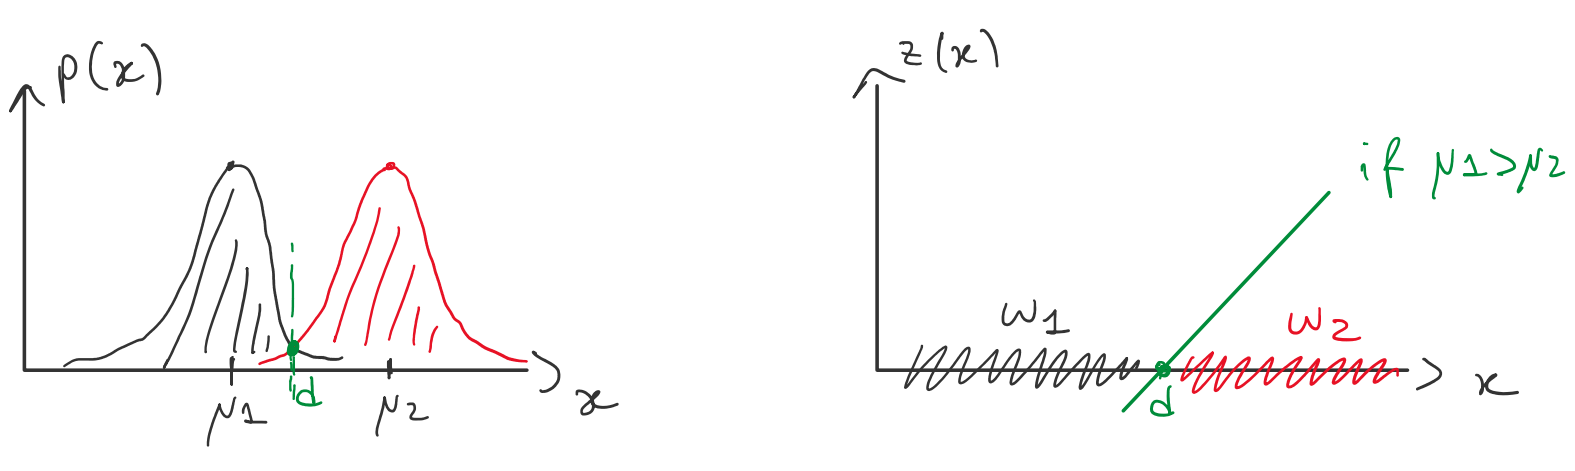
\includegraphics[scale=0.45]{C_1_1}
        \centering
    \end{figure}
    \item \(h>1\Rightarrow\sigma_1^2<\sigma_2^2\): the Gaussian distribution of \(w_1\)
    has a smaller variance, thus it is steeper, while \(w_2\) is wider, the polynomial \(z(x)\)
    is of 2nd order and the sign in front of \(x^2\) is negative, thus the
    positive portion of the parabula indicates the interval on the variable \(x\)
    which would select the class \(w_1\).
    \begin{figure}[H]
        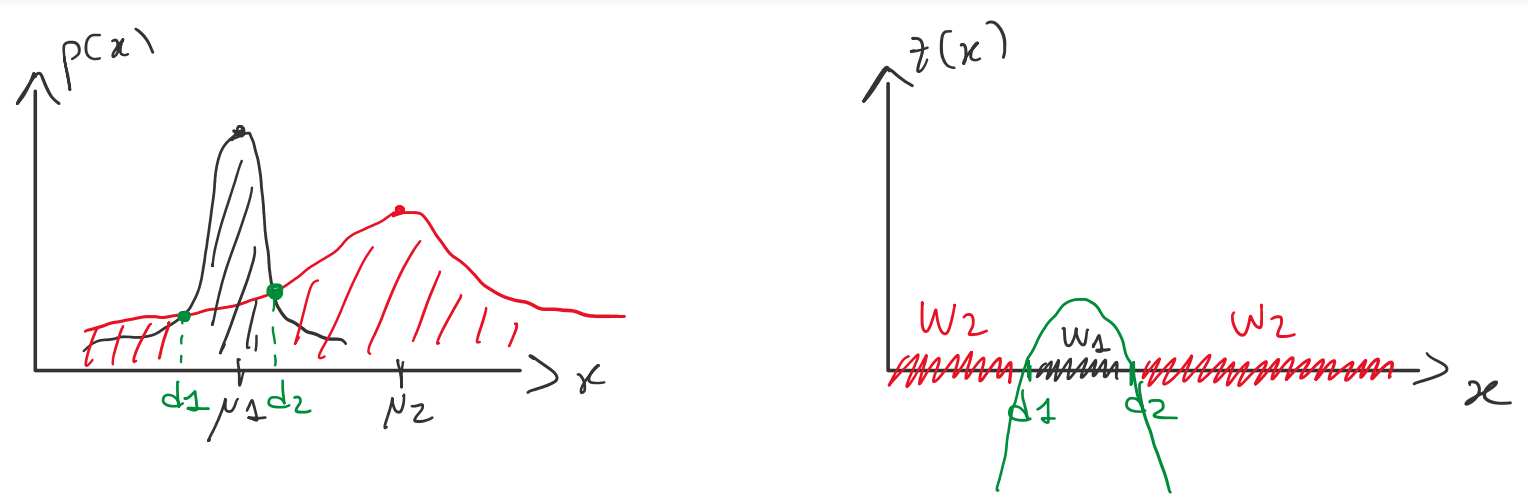
\includegraphics[scale=0.45]{C_1_2}
        \centering
    \end{figure}
    \item \(h<1\Rightarrow\sigma_1^2>\sigma_2^2\): the Gaussian distribution of \(w_1\)
    has a larger variance, thus it is wider, while \(w_2\) is steeper, the polynomial \(z(x)\)
    is of 2nd order and the sign in front of \(x^2\) is positive, thus the
    negative portion of the parabula indicates the interval on the variable \(x\)
    which would select the class \(w_2\).
    \begin{figure}[H]
        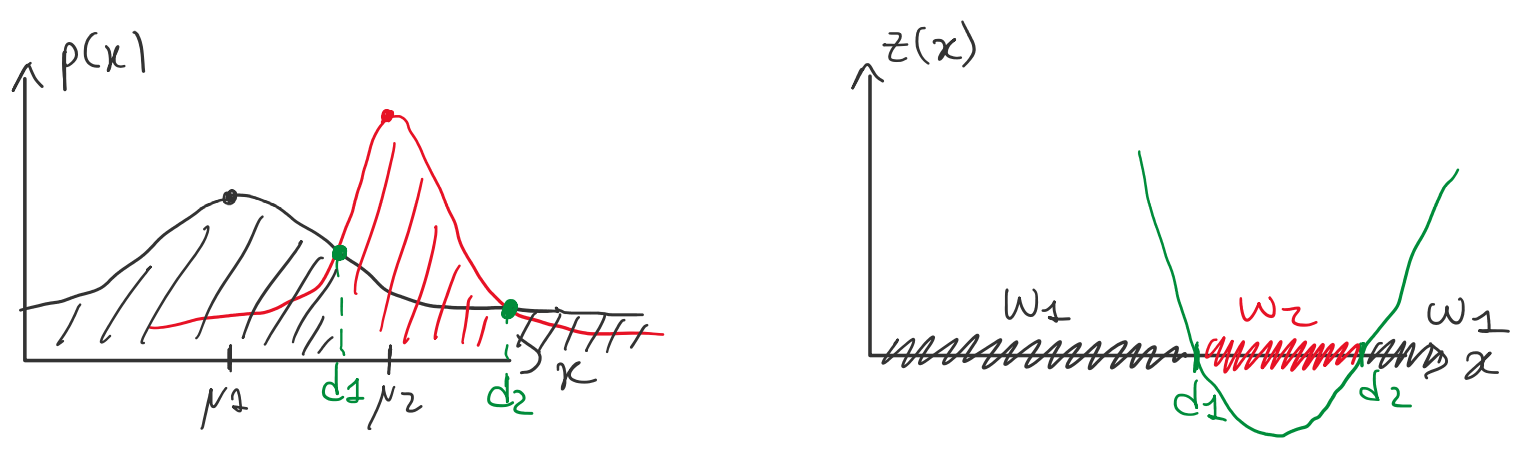
\includegraphics[scale=0.45]{C_1_3}
        \centering
    \end{figure}
  \end{enumerate}